% $Header$

\documentclass{beamer}

% Copyright (c)  2021  HiKlas Ltd.
% Permission is granted to copy, distribute and/or modify this document
% under the terms of the GNU Free Documentation License, Version 1.3
% or any later version published by the Free Software Foundation;
% with no Invariant Sections, no Front-Cover Texts, and no Back-Cover Texts.
% A copy of the license is included in the section entitled "GNU
% Free Documentation License".
%
% Based on the Beamer generic-ornate-15min-45min.en.tex template by
% Till Tantau <tantau@users.sourceforge.net>



\mode<presentation>
{
  \usetheme{CambridgeUS}
}

\usepackage[english]{babel}
\usepackage[latin1]{inputenc}
\usepackage[T1]{fontenc}
% Or whatever. Note that the encoding and the font should match. If T1
% does not look nice, try deleting the line with the fontenc.

% These packages are used for drawing circuits
\usepackage{tikz}
\usepackage[siunitx,european,americanresistors]{circuitikz}

% Packages for mathematical notation
\usepackage{amsmath}

% Trying to split long URLs across lines
% From this post suggesting breakurl: https://stackoverflow.com/questions/2640111/url-latex-linebreak
% The breakurl package: https://ctan.org/pkg/breakurl?lang=en
% Example of options: https://tex.stackexchange.com/questions/298851/linebreak-in-long-url-breakurl-wont-break-it
\usepackage{hyperref}
\usepackage[hyphenbreaks]{breakurl}

% Information about the presentation 
\title{Introduction to Machine Code}
\subtitle{002 Processors}
\author{Fiona Bianchi}
\institute{HiKlas Ltd}
\date{August 2021}
\subject{Talks}
\pgfdeclareimage[height=0.5cm]{company-logo}{../assets/HiklasLogo.eps}
\logo{\pgfuseimage{company-logo}}

% Table of contents for each Subsection
\AtBeginSubsection[]
{
  \begin{frame}<beamer>{Outline}
    \tableofcontents[currentsection,currentsubsection]
  \end{frame}
}

% TODO: Nope, I don't think I want this put leaving it in just in case
% TODO: to remove when absolutely sure
% If you wish to uncover everything in a step-wise fashion, uncomment
% the following command: 
%\beamerdefaultoverlayspecification{<+->}

% Show the notes
\ifdefined\isnotes
\setbeameroption{show only notes}
\fi

% Show notes and slides
\ifdefined\ishandout
\setbeameroption{show notes}
\fi


\begin{document}

\begin{frame}
  \titlepage
\end{frame}

\begin{frame}{Outline}
  \tableofcontents
  % TODO: What is "pausesections" for?
  % You might wish to add the option [pausesections]
\end{frame}

\section{What do processors look like?}

\subsection[Precursors]{Very old}

\begin{frame}{Babbage Difference Engine}
  \begin{columns}
    \column{0.5\textwidth}

    \begin{itemize}
    \item
      Designed by Charles Babbage \cite{BabbageBio}
      \note[item]{Implementation of No.0 and partial No.1}
      \note[item]{Designed No.2 Difference Engine}
      \note[item]{No.0 was completed in 1822}
    \item
      Completely mechanical calculating engine 
    \item
      Superseded in design by analytical engine \cite{AnalyticalEngine}
      \note[item]{Only designed never implemented in Babbage's lifetime}
      \note[item]{General purpose computer design with processor, memory}
      \note[item]{ALU - Arithmetic and Logic unit: tests, branches, loops}
      
    \end{itemize}

    \column{0.50\textwidth}
    \begin{center}
      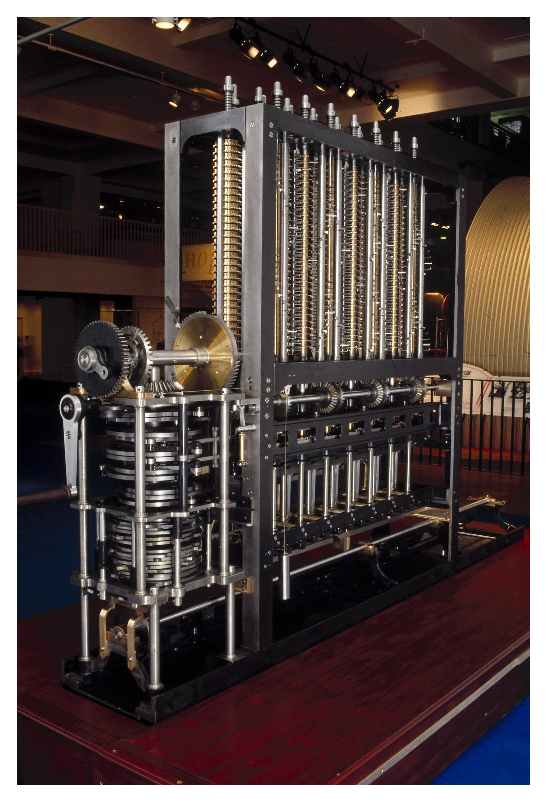
\includegraphics[scale=0.4]{../assets/Difference_Engine_London.eps}
      \cite{BabbageEngine} Difference Engine No.2
    \end{center}

  \end{columns}
\end{frame}


\subsection[Firsts]{Old}

\begin{frame}{Colossus}
  \begin{columns}
    \column{0.5\textwidth}
    
    \begin{itemize}
    \item
      World's first* Programmable computer
      \note[item]{Originally this was thought to be ENIAC before Bletchley Park secrets revealed}
      \note[item]{Colossus was destoryed at the end of WWII and plans might have made it across to US}
      \note[item]{There may be German and other programmable computers that pre-date Colossus}
    \item
      Used for code-breaking at Bletchley Park
    \item
      Paper tape used as input for the program and data
      \note[item]{Punched tape and cards continuted to be used for many years}
      \note[item]{Data read using light source and sensors that could detect punched hole}
    \end{itemize}
    
    \column{0.50\textwidth}
    \begin{center}
      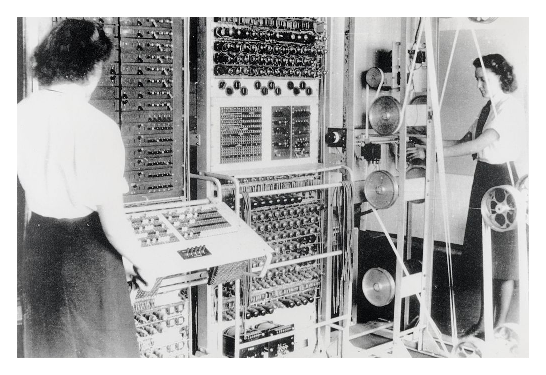
\includegraphics[scale=0.6]{../assets/ColossusOperation.eps}
      \cite{Colossus1943} Colossus Operating in 1943
    \end{center}
    
  \end{columns}
\end{frame}

\begin{frame}{Colossus Rebuild}
  \begin{columns}
    \column{0.55\textwidth}
    
    \begin{itemize}
    \item
      Rebuilt at [TNMOC] by a team including some of the original engineers
    \item
      Makes use of relays and valves
      \note[item]{Valves are an electronic device that uses heated electrodes and electrons}
      \note[item]{Valves use similar principles to that in CRT, Cathode Ray Tubes in old TVs}
      \note[item]{Valves were a precussor to transitors, although the latter use totally different mechanism}
    \item
      On display at [TNMOC] and fully working
    \end{itemize}
    
    \column{0.45\textwidth}
    \begin{center}
      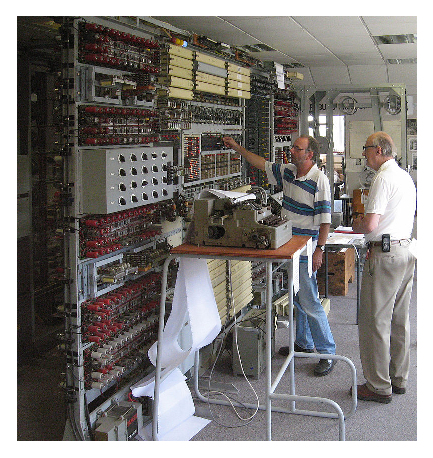
\includegraphics[scale=0.75]{../assets/ColossusRebuild_11.eps}
      \cite{ColossusRebuild}
    \end{center}
    
  \end{columns}
\end{frame}


\subsection[Modern]{Current}

\begin{frame}{Integrated Circuits}
  \begin{columns}
    \column{0.50\textwidth}
    
    \begin{itemize}
    \item
      Invention of the \cite{Transistor} in 1947
    \item
      Invention of \cite{ICs} in the 1960s
    \item
      Very Large Scale Integration, \cite{VLSI}, 1970s
    \item
      VLSI pioneer, \cite{LynnConway}
      \note[item]{Invented generalised dynamic instruction handling}
      \note[item]{Mead-Conway design revolution}
      \note[item]{Originally fired by IBM when she transitioned in 1968}
      \note[item]{IBM officially and publically apologised in 2020}
    \item
      Processors in silicon integrated circuits
    \item
      Leading to home microcomputers
    \end{itemize}
    
    \column{0.50\textwidth}
    \begin{center}
      \includegraphics[scale=0.25]{../assets/MOS_6502_Die.eps}
      \cite{MOS6502Die}
    \end{center}
    
  \end{columns}
\end{frame}


\begin{frame}{BBC Micro}
  \begin{columns}
    \column{0.50\textwidth}
    
    \begin{itemize}
    \item
      Released in 1981
      \begin{itemize}
      \item
        6502 CPU clocked at 2Mhz (see later)
      \item
        32Kb RAM
      \item
        32Kb ROM (slightly less)
      \item
        Storage on cassette tape, floppy disk (5 1/4, then 3 1/2), Winchester harddrive
      \end{itemize}
    \item
      Later models
      \begin{itemize}
      \item
        Acorn Electron
      \item
        BBC Master 128
      \item
        Acorn Archimedies
        \note[item]{This is a radical change that has led to much of our modern technology}
        \note[item]{The ARM processor is used in phones, tablets, and now laptops including Apple M1/M2}
      \end{itemize}
    \end{itemize}
    
    \column{0.50\textwidth}
    \begin{center}
      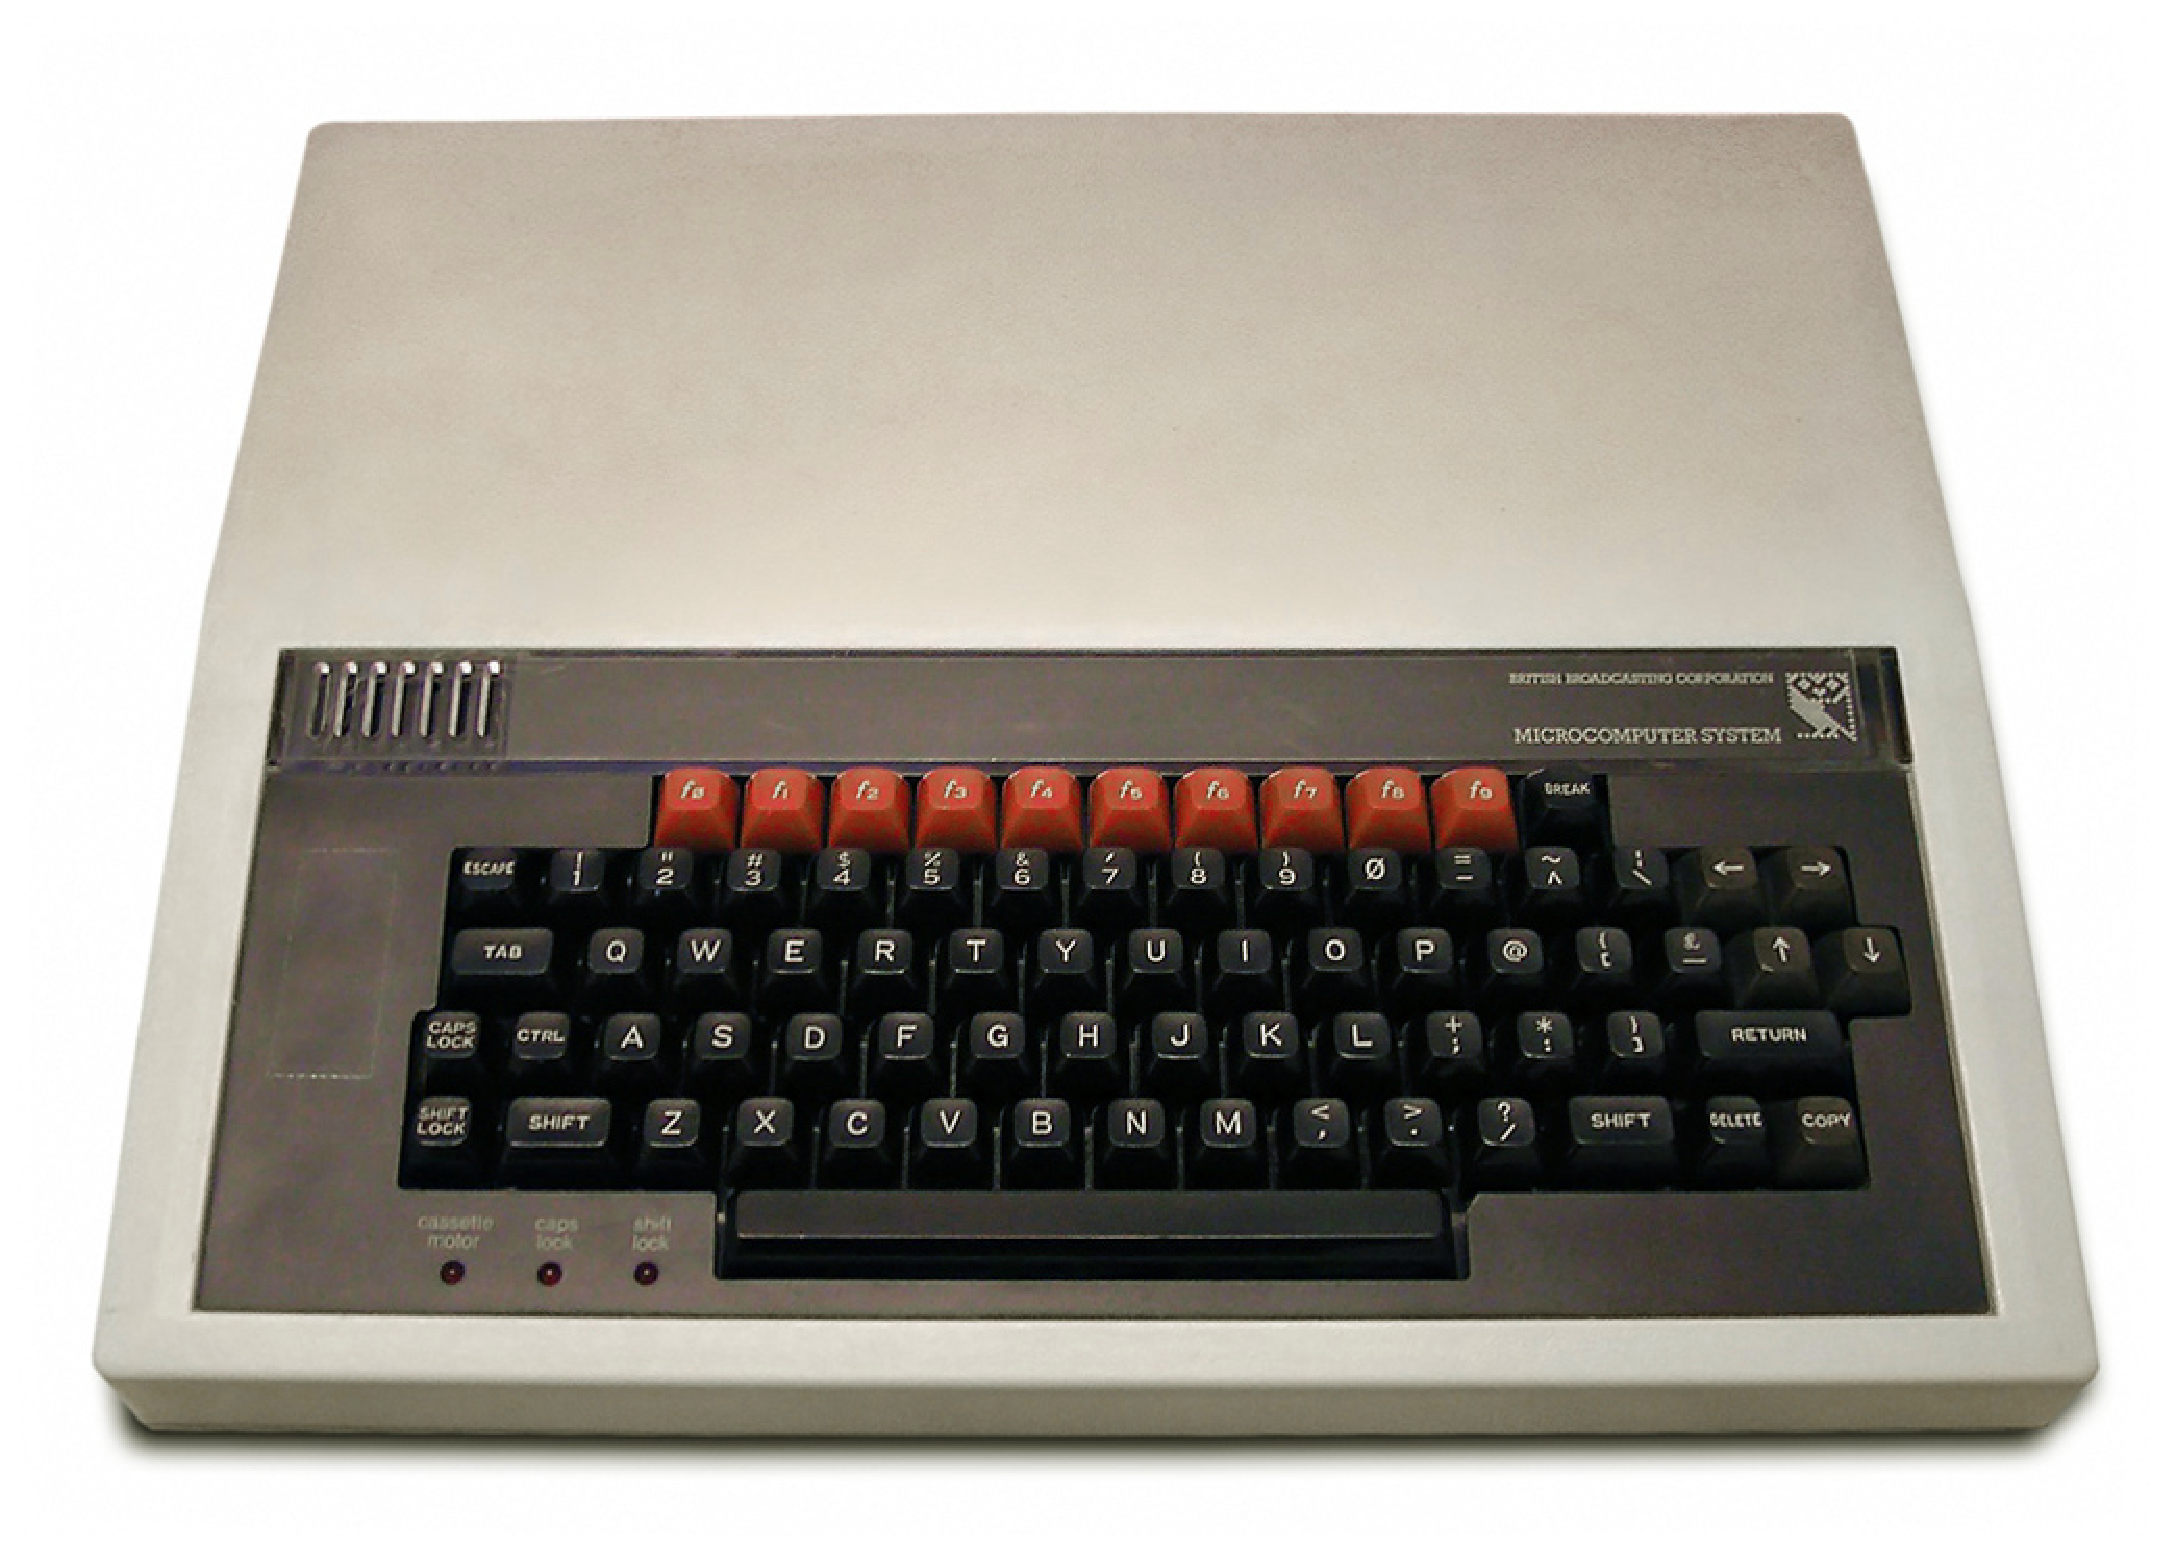
\includegraphics[scale=0.15]{../assets/BBC_Micro_Front_Restored.eps}
      \cite{BBCMicro}
    \end{center}
    
  \end{columns}
\end{frame}



\section{What do processors do?}

\subsection[Maths]{Simple maths}

\begin{frame}{Whole Numbers}
  \begin{itemize}
  \item
    Addition, Subtraction, Multiplication, Division
  \item
    Add/Subtract easy in hardware
  \item
    Multiply/divide more complicated
  \item
    Fixed sized numbers, 8bit, 16bit, 32bit, 64bit
  \end{itemize}
\end{frame}

\begin{frame}{Logical Operations}
  \begin{itemize}
  \item
    Again fixed size numbers
  \item
    Operations on binary bits
  \item
    AND, OR, XOR, NOT
  \item
    Used for transforming or manipulating data (bitmasks for example)
  \end{itemize}
\end{frame}

\begin{frame}{Comparisons and Tests}
  \begin{itemize}
  \item
    Greater than, less than, equal to zero
  \item
    Used as conditions on branches, e.g. branch if not zero
  \item
    Uses basic maths operations, e.g. subtract
  \item
    Maths operations can trigger carry flag
  \end{itemize}
\end{frame}


\subsection[Memory]{Remembering Data}

\begin{frame}{Types of Memory}
  \begin{itemize}
  \item
    Registers: inside the processor
  \item
    Cache: also often on the same die as the CPU
  \item
    RAM: Random Access Memory - read/write
    \begin{itemize}
    \item
      Static RAM (SRAM)
    \item
      Dynamic RAM (DRAM)
    \end{itemize}
  \item
    ROM: Read Only memory
    \begin{itemize}
    \item
      EPROM: Erasable Programmable Read Only Memory
    \item
      EEPROM: Electrically Eraseable
    \end{itemize}
  \end{itemize}
\end{frame}

\subsection[IO]{Input/Output}

\begin{frame}{A frame}
  \begin{itemize}
  \item
    One item
  \item
    Two item
  \end{itemize}
\end{frame}

\section{Programming Processors}

\subsection[Older]{Beginnings}

\begin{frame}{A frame}
  \begin{itemize}
  \item
    One item
  \item
    Two item
  \end{itemize}
\end{frame}

\subsection[Assembly]{Assembly Language}

\begin{frame}{A frame}
  \begin{itemize}
  \item
    One item
  \item
    Two item
  \end{itemize}
\end{frame}


\subsection[Compilers]{Compilers}

\begin{frame}{A frame}
  \begin{itemize}
  \item
    One item
  \item
    Two item
  \end{itemize}
\end{frame}





\section{Summary}

\begin{frame}{Summary}

  % Keep the summary *very short*.
  \begin{itemize}
  \item
    Item one
  \item
    Item two
  \end{itemize}
  
  % The following outlook is optional.
  \vskip0pt plus.5fill
  \begin{itemize}
  \item
    Outlook
    \begin{itemize}
    \item
      Something you haven't solved.
    \item
      Something else you haven't solved.
    \end{itemize}
  \end{itemize}
\end{frame}


\section{Bibliogrphy}

\begin{frame}{Bibliography 1}
  \frametitle{References}
  
  \begin{thebibliography}{Babbage Difference Engine}
  \bibitem[Babbage Difference Engine]{BabbageEngine}
    Science Museum London, Difference Engine No.2
    \newblock {\url{https://collection.sciencemuseumgroup.org.uk/objects/co526657/difference-engine-no-2-designed-by-charles-babbage-built-by-science-museum-difference-engine}}

  \bibitem[Babbage Biography]{BabbageBio} 
    Charles Babbage Biography with references
    \newblock {\url{https://mathshistory.st-andrews.ac.uk/Biographies/Babbage/}}

  \bibitem[Analytical Engine]{AnalyticalEngine}
    Babbage Analytical Engine
    \newblock {\url{https://en.wikipedia.org/wiki/Analytical_Engine}}

  \bibitem[Colossus]{Colossus}
    The rebuild colossus at \cite{TNMOC} TNMOC
    \newblock {\url{https://www.tnmoc.org/colossus}}

  \end{thebibliography}
\end{frame}

\begin{frame}{Bibliography 2}
  \frametitle{References}
  
  \begin{thebibliography}{ColossusRebuild}
  \bibitem[TNMOC]{TNMOC}
    The National Museum Of Computing
    \newblock {\url{https://www.tnmoc.org/}}
    
  \bibitem[Bletchley Park]{Bletchley}
    Bletchley Park
    \newblock {\url{https://bletchleypark.org.uk}}
    
  \bibitem[Colossus Operation]{Colossus1943}
    Colossus being operated by Dorothy Du Boisson (left) and Elsie Booker (right)
    \newblock {\url{https://en.wikipedia.org/wiki/Colossus_computer\#/media/File:Colossus.jpg}}

  \bibitem[Colossus Rebuild]{ColossusRebuild}
    Rebuild of Colossus supervised by Tony Sale (Right)
    \newblock {\url{https://en.wikipedia.org/wiki/Colossus_computer\#/media/File:ColossusRebuild_11.jpg}}
  \end{thebibliography}
\end{frame}



\begin{frame}{Bibliography 3}
  \frametitle{References}
  
  \begin{thebibliography}{BBC Microcomputer}
  \bibitem[Transistor]{Transistor}
    The Invention of the transistor on 1947
    \newblock {\url{https://en.wikipedia.org/wiki/Transistor}}
  \bibitem[Integrated Circuits]{ICs}
    Integrated Circuits from the 1960s
    \newblock {\url{https://en.wikipedia.org/wiki/Transistor}}
  \bibitem[VLSI]{VLSI}
    VLSI Circuits
    \newblock {\url{https://en.wikipedia.org/wiki/Very_Large_Scale_Integration}}
  \bibitem[Lynn Conway]{LynnConway}
    Lynn Conway
    \newblock {\url{https://en.wikipedia.org/wiki/Lynn_Conway}}
  \bibitem[MOS 6502 Die]{MOS6502Die}
    Die image
    \newblock {\url{https://commons.wikimedia.org/wiki/File:MOS_6502_die.jpg}}
  \bibitem[BBC Microcomputer]{BBCMicro}
    The BBC Microcompter from Acorn Computers
    \newblock {\url{https://en.wikipedia.org/wiki/BBC_Micro\#/media/File:BBC_Micro_Front_Restored.jpg}}
  \end{thebibliography}
\end{frame}

\end{document}
